% Requesting draft will show any overfull boxes when the document is compiled. Should be black lines on the document where the boxes are overfull.
\documentclass{refrep}
%\usepackage[textsize=tiny]{todonotes}
\usepackage{listings}  % See https://www.sharelatex.com/learn/Code_listing#Importing_code_from_a_file to read about how to showcase python code in this manual.
\usepackage{todonotes}
\usepackage[utf8]{inputenc}
%Commented these out b/c they don't seem to be necessary to put a caption beneath tables. if the spacing gets messed up, try un-commenting them.
%\usepackage{caption}
%\captionsetup[table]{position=bottom}
\usepackage{url}
\usepackage{graphicx}  % This package lets you import images into the document.
\graphicspath{ {BioPype_images/} }  % Specify the path to the folder where the images will be imported from.
\usepackage[toc,page]{appendix}

% This is to stop the individual appendix entries from appearing in the ToC.
\usepackage{etoolbox}
\appto\appendix{\addtocontents{toc}{\protect\setcounter{tocdepth}{0}}}
% reinstate the correct level for list of tables and figures
\appto\listoffigures{\addtocontents{lof}{\protect\setcounter{tocdepth}{1}}}
\appto\listoftables{\addtocontents{lot}{\protect\setcounter{tocdepth}{1}}}

\usepackage{hyperref}  % Allows hyperlinks.

\title{BioPype: A crash course in bioinformatics and custom pipelines}

\author{Ethan Gniot}
\date{March 2018}

\begin{document}

\maketitle 
\listoftodos
\tableofcontents % This creates the table of contents; autofills Chapters, sub-chapters (aka "sections"), and page numbers.

% Add an asterisk before the {} to make an un-numbered chapter that won't be included in the ToC.
\chapter{Foreword}

\section{Goal}
This tutorial aims to improve your general understanding of bioinformatics through several methods:
\begin{itemize}
    \item Define technical terms commonly used in bioinformatics methods and found in the literature.
    \item Provide a collection of various useful resources, including...
    \begin{enumerate}
        \item Resources for finding tools, data, and background information that can help answer your research questions.
        \item Resources that explain details about bioinformatics concepts and techniques in beginner-friendly language.
    \end{enumerate}
    \item Demonstrate how Python can be used to answer your research questions by combining existing bioinformatics tools and automating repetitive or time-consuming tasks.
\end{itemize}

\section{How to use this book}
Most reference materials are consolidated in the appendices at the end of the book. The main text of this book is written in the right-hand margin. The left-hand margin contains special markers and important notes to the reader. The book can be used as a self-paced tutorial with the help of the markers described below.

------------------------------- 

\textit{Lorem ipsum dolor sit amet, consectetur adipiscing elit. Maecenas eu felis sodales, interdum purus nec, interdum ex. Integer at nunc \marginlabel{This is a margin label. I will write things here to further explain the main text, define jargon, etc.} ultricies, tempus nibh eget, egestas risus. Suspendisse aliquam, lorem at dictum accumsan, dolor elit euismod velit, a gravida risus libero non felis. Donec a tortor tempor, scelerisque sapien posuere, volutpat erat. Morbi in imperdiet velit. Vivamus sagittis, massa sit amet venenatis euismod, elit eros aliquam diam, molestie faucibus lectus nisi euismod erat. Nulla id dictum mi.}

\attention \textbf{The arrow that points to this line is an "Attention" marker. It will indicate key pieces of information that you should pay special attention to.} \textit{Curabitur egestas aliquam nisl, pharetra finibus mauris placerat nec. Nam in diam risus. Nulla mollis purus quis feugiat tristique. Vestibulum et sollicitudin ante, at sagittis ipsum. Nunc hendrerit ante sed massa semper eleifend.}

\seealso{This kind of annotation will reference appendix entries that you can consult for more-detailed information about the main text.} Ut ultrices eros velit, at faucibus ante rutrum eget. Pellentesque a molestie diam. Curabitur mattis dui a risus lacinia fringilla. Phasellus porttitor elit nec neque euismod, id ultrices elit lobortis. Aliquam molestie sem. Curabitur sit amet urna faucibus, vulputate arcu sit amet, fermentum ipsum. Nulla facilisi. Nam ullamcorper eget leo id malesuada.

\section{Pre-requisites}
\subsection*{Things to know}
\subsection*{Computer requirements}
\begin{itemize}
    \item At least 4GB RAM bare minimum, 16GB RAM if possible (basically, the more RAM, the better)
    \item Must be able to run macOS 10.12 Sierra, preferably macOS 10.13 High Sierra
    \item At least 500GB storage (ideally several TB)
\end{itemize}

\chapter{Source Code}
(Source code can be found at github.com/EthanGniot/LU-microbiome)

\chapter{Sample Information}
\todo{Still need to add information about the inflammatory bowel disease dataset}

While we are building the LU-microbiome pipeline, we will need a dataset that we can use to test our pipeline throughout the process and make sure it is working as intended. In order to do this, we must use a dataset that's already been analyzed so that we know what the results should look like. When we test our pipeline, if our results match the results of the original analysis, then we will know that our tool is working correctly.

There are several test datasets available to us for testing the feature that analyzes the relative abundance of bacteria in the microbiota.

The first is the dataset used in both the QIIME ``Illumina Overview Tutorial" (\ref{appendix:IlluminaOverTut}) \todo{Make URLs footnotes instead of appendix entries} and the QIIME 2 ``Moving Pictures" tutorial (\ref{appendix:MovingPicTut}) derived from the \seealso{Caporaso et al, 2011 \cite{Caporaso2011}} \textit{Moving Pictures of the Human Microbiome} study, where two human subjects collected daily samples from four body sites: the tongue, the palm of the left hand, the palm of the right hand, and the gut (via fecal samples obtained by swapping used toilet paper). These data were sequenced using the barcoded amplicon sequencing protocol described in \seealso{ THIS CITATION NEEDS TO BE FIXED \cite{Caporaso2011a}} \textit{Global patterns of 16S rRNA diversity at a depth of millions of sequences per sample}. A more recent version of this protocol that can be used with the Illumina HiSeq 2000 and MiSeq can be found here. \todo{Fix bibliography entries in this paragraph and in general. They're not correctly referencing even though bib file has entries.}

(Here is information about the untested inflammatory bowel disease dataset that we will analyze using the completed pipeline)

\chapter{Setting the scene}
("Here" is a hypothetical situation/research question that a student may have. This is the research question that will be answered by the pipeline we are creating.)

\chapter{Microbiome Analysis}
(This chapter will give some general background information about the topics listed below. More-detailed information will be provided in later chapters when we are actually creating the pipeline)
\section{The Gut Microbiome}
\section{Relative Abundance Analysis}
\section{Metagenomics}
\section{Python}

\chapter{How to Find Tools}
\section{Finding Data}
(Here is where we talk about various databases that users can use to find general information, data files, study results, public datasets, etc.)
\section{Finding Software}
(Here is where we talk about ways/places that people can look for software programs that can help answer their research question.)

% 1) Delete all aux files.
% 2) Comment out all appendix sections and labels. Save file.
% 3) Compile main tex file x2
% 4) Un-comment all appendix sections and labels. Save file.
% 5) Compile main tex file x2

\chapter{Plan: 8 Main Sections}
(Break down the sub-tasks required to accomplish the two main tasks: Relative abundance analysis and metagenomic analysis)
%
\begin{enumerate}
    \item What is my research question?
    \item Is there an existing tool that I can use to directly answer my research question? If not, proceed to Step 3.
    \item What is the step-by-step process required to answer my research question?
    \item What existing tools are available that can help me accomplish each of these steps?
    \item How do I write code that uses these tools to accomplish the steps?
\end{enumerate}
%

\chapter{Software and Set-up}
\label{chap:software}
\section{Software}
(Table of software name, name in PATH, version number, function of the software for each one we're gonna use)
\todo{Add further software that you end up using (e.g., USEARCH). ALSO, make sure to update the section that mentions installing packages if you do so.}
\todo[inline]{add 3rd column to table with link to documentation/download source}
%
\begin{table}[htp]
    \begin{center}
    \begin{tabular}{ l | l }
        \textit{Software name} & \textit{Version number} \\ 
        \hline
        Anaconda & 5.1 \\  
        Biopython & 1.70 \\
        BLAT & 35 \\
        matplotlib & 2.2.2 \\
        pandas & 0.22.0 \\
        sra-tools & 2.8.2 \\
        trim-galore & 0.4.5 \\
    \end{tabular}
    \caption{\textbf{Software used to create the tutorial pipeline.}}
    \label{tab:software}
    \end{center}
    \label{software}
\end{table}
%
\section{Set-up and Install Dependencies}
Before we write any code, there are several steps that must be completed to prep your machine for the tasks we will be performing in this tutorial. Without these prerequisites, the code you write during this tutorial will not work correctly:
\begin{enumerate}
\item Install and open Anaconda
\item Create a new virtual environment
\item Install packages
\end{enumerate}

\subsection{Install Anaconda}
The Anaconda program will play a key role in this tutorial. Anaconda is essentially Python and a lot of scientific computing tools bundled together, along with many popular add-ons to Python called packages. \seealso{RESOURCE FOR LEARNING ABOUT PYTHON PACKAGES} Downloading all of these tools individually can be difficult, as the quirks of one package may conflict with another when they're installed manually; using Anaconda to install packages greatly simplifies the process because Anaconda can smoothly handle all of the minute details that cause manual installations to fail.

\textbf{\underline{Install and Open:}}

\begin{enumerate}
    \item Go to the download page for the Anaconda distribution at \\ \url{https://www.anaconda.com/download}. 
    \item Select your preferred operating system from the Windows, macOS, or Linux tabs, then select the Download option for the \textbf{Python 3.6 version} (Figure \ref{anaconda_download}) and follow the installation instructions.
    %
    \begin{figure}[h]
        \begin{center}
        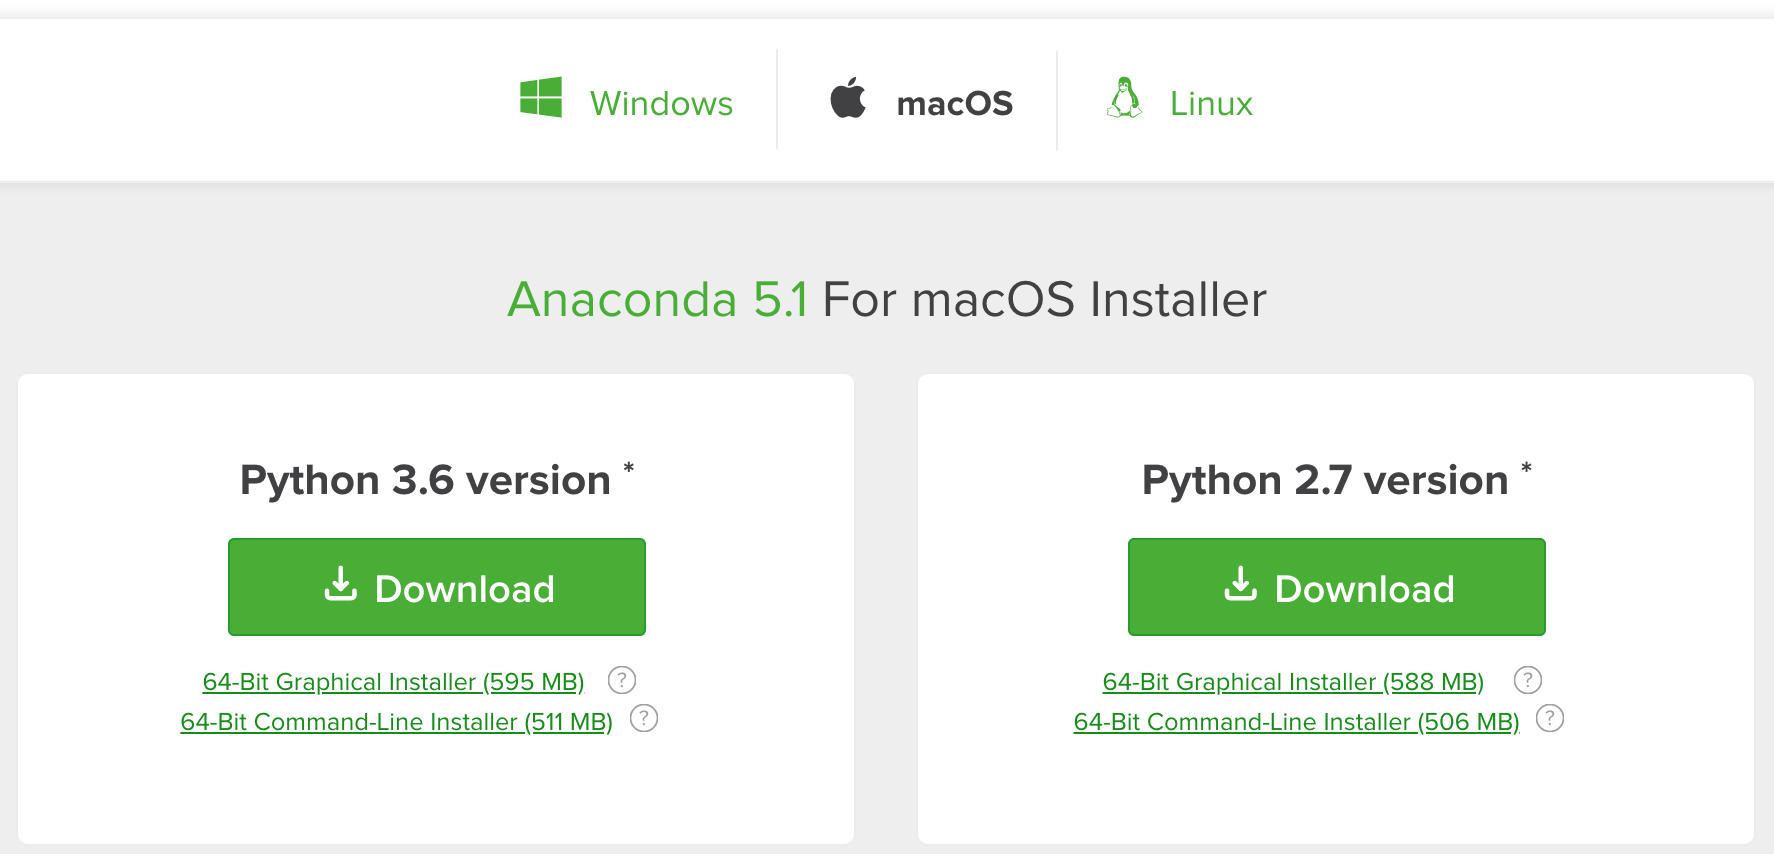
\includegraphics[width=9.5cm]{anaconda_download}
        \caption{The Anaconda download options provided on the Anaconda distribution website at \protect \url{https://www.anaconda.com/download}}.
        \label{anaconda_download}
        \end{center}
    \end{figure}
    %


    \item After installation is complete, open the application named ``Anaconda-Navigator" (the icon looks like 
\includegraphics[width=0.5cm]{anaconda-navigator-thumbnail}). After a brief start-up period, you should see the following window (Figure \ref{anaconda-nav-win}):
    %
    \begin{figure}[htbp]
        \begin{center}
        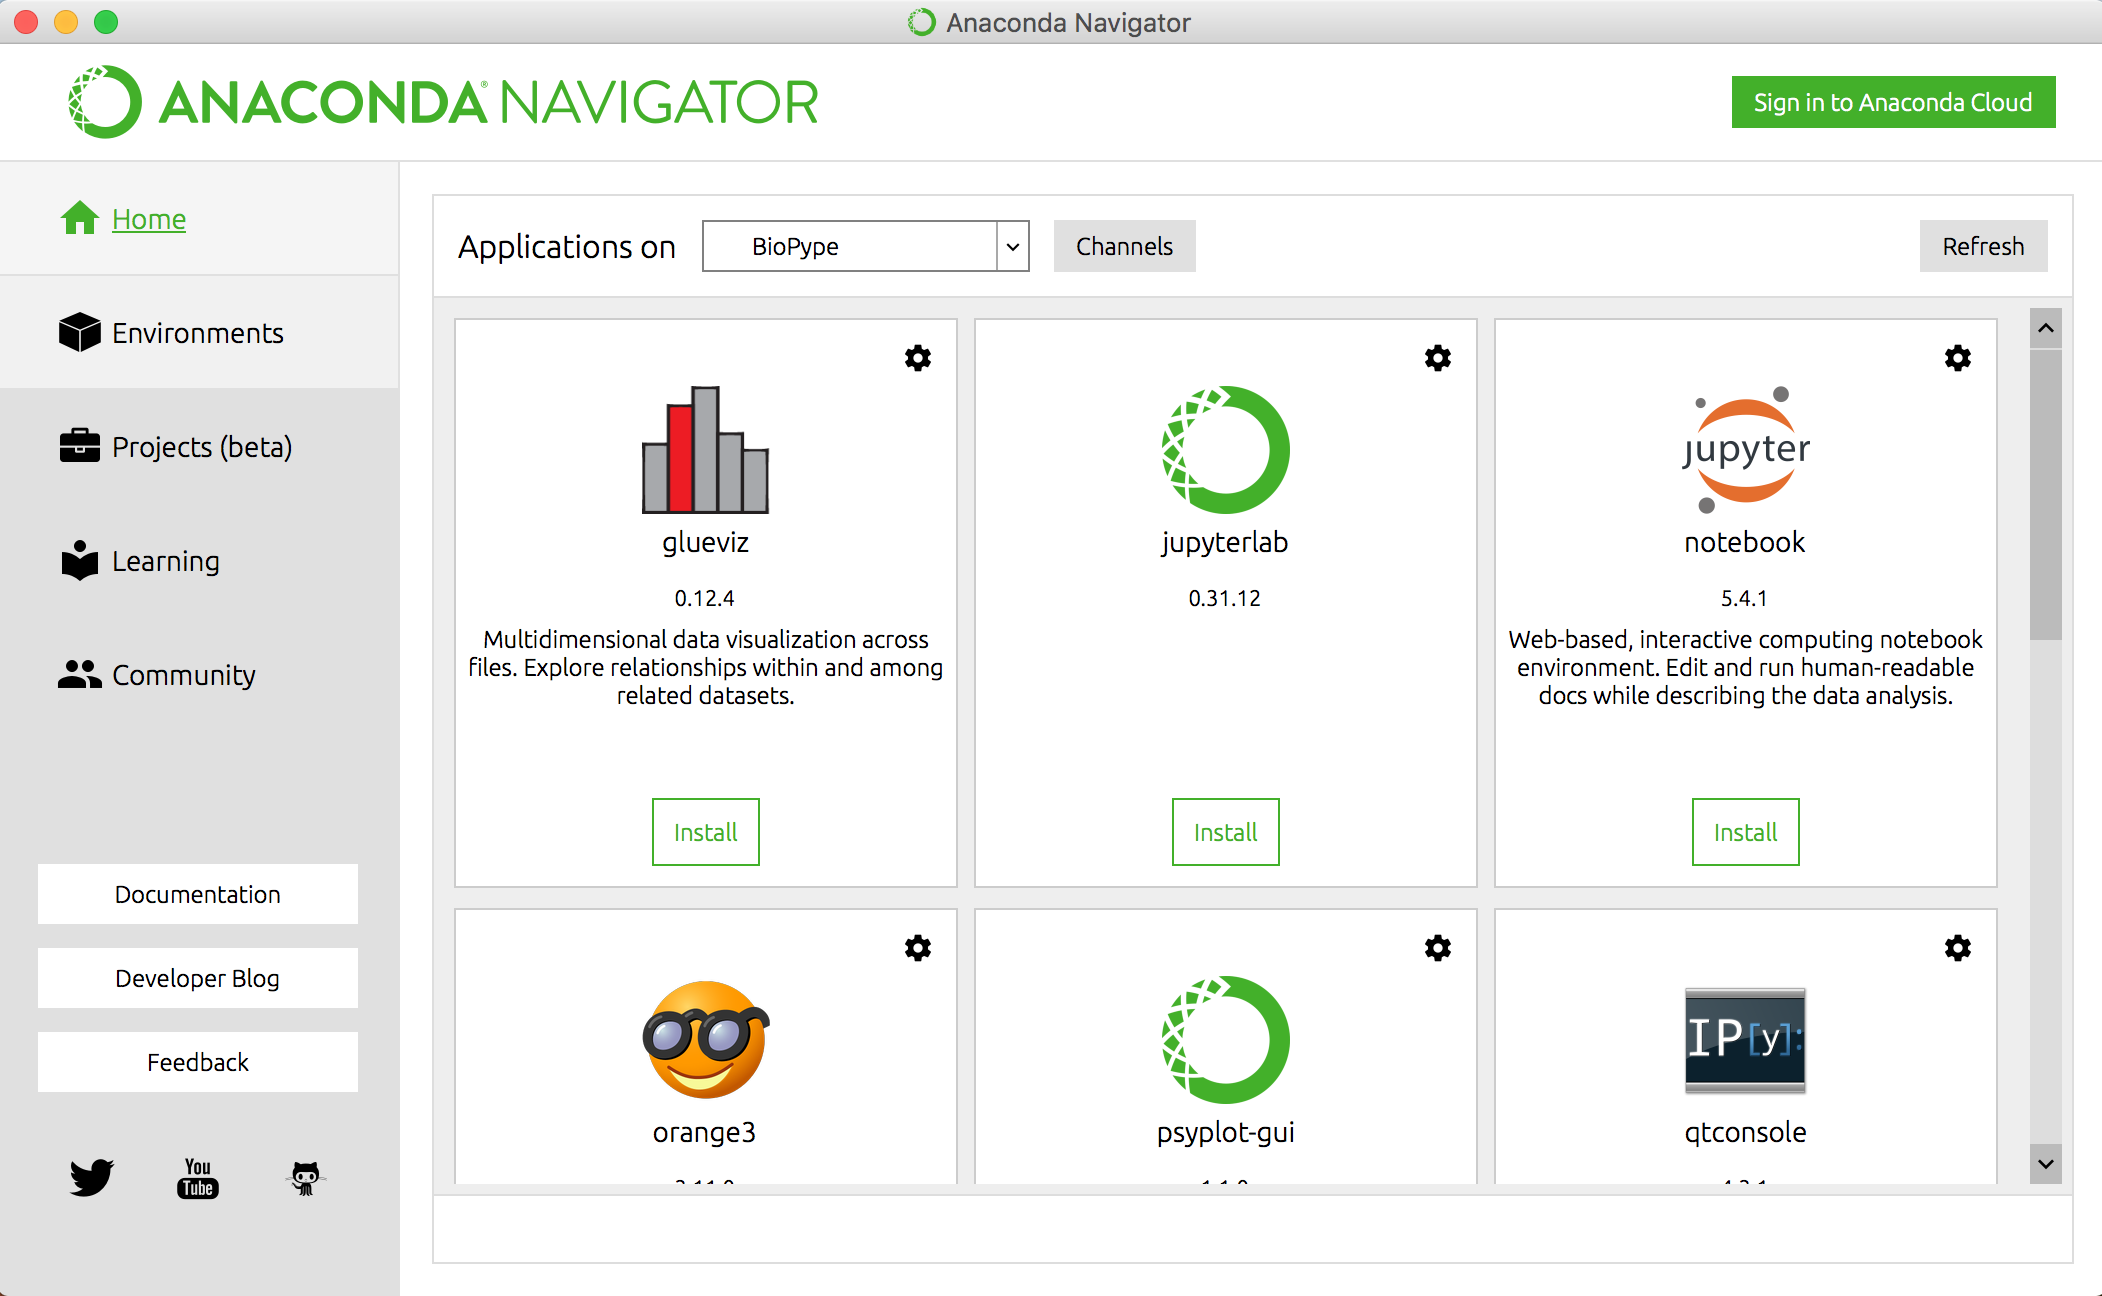
\includegraphics[width=12cm]{anaconda-nav-win}
        \caption{The window displayed to the user upon opening Anaconda-Navigator.}
        \label{anaconda-nav-win}
        \end{center}
    \end{figure}
    %
\end{enumerate}

\subsection{Create a New Virtual Environment}
    \todo[inline]{Write a blurb explaining the benefits of using a virtual environment.}
    \todo[inline]{Link to resource for further reading on virtual environments}
    \marginlabel{Make sure the computer has an internet connection while completing this section, otherwise Anaconda will not let you create a virtual environment.}
    \begin{enumerate}
        \item On the left side of the Anaconda-Navigator window, click on the tab labeled \textbf{Environments}. (Figure \ref{anaconda-env-win}) 
        %
        \begin{figure}
            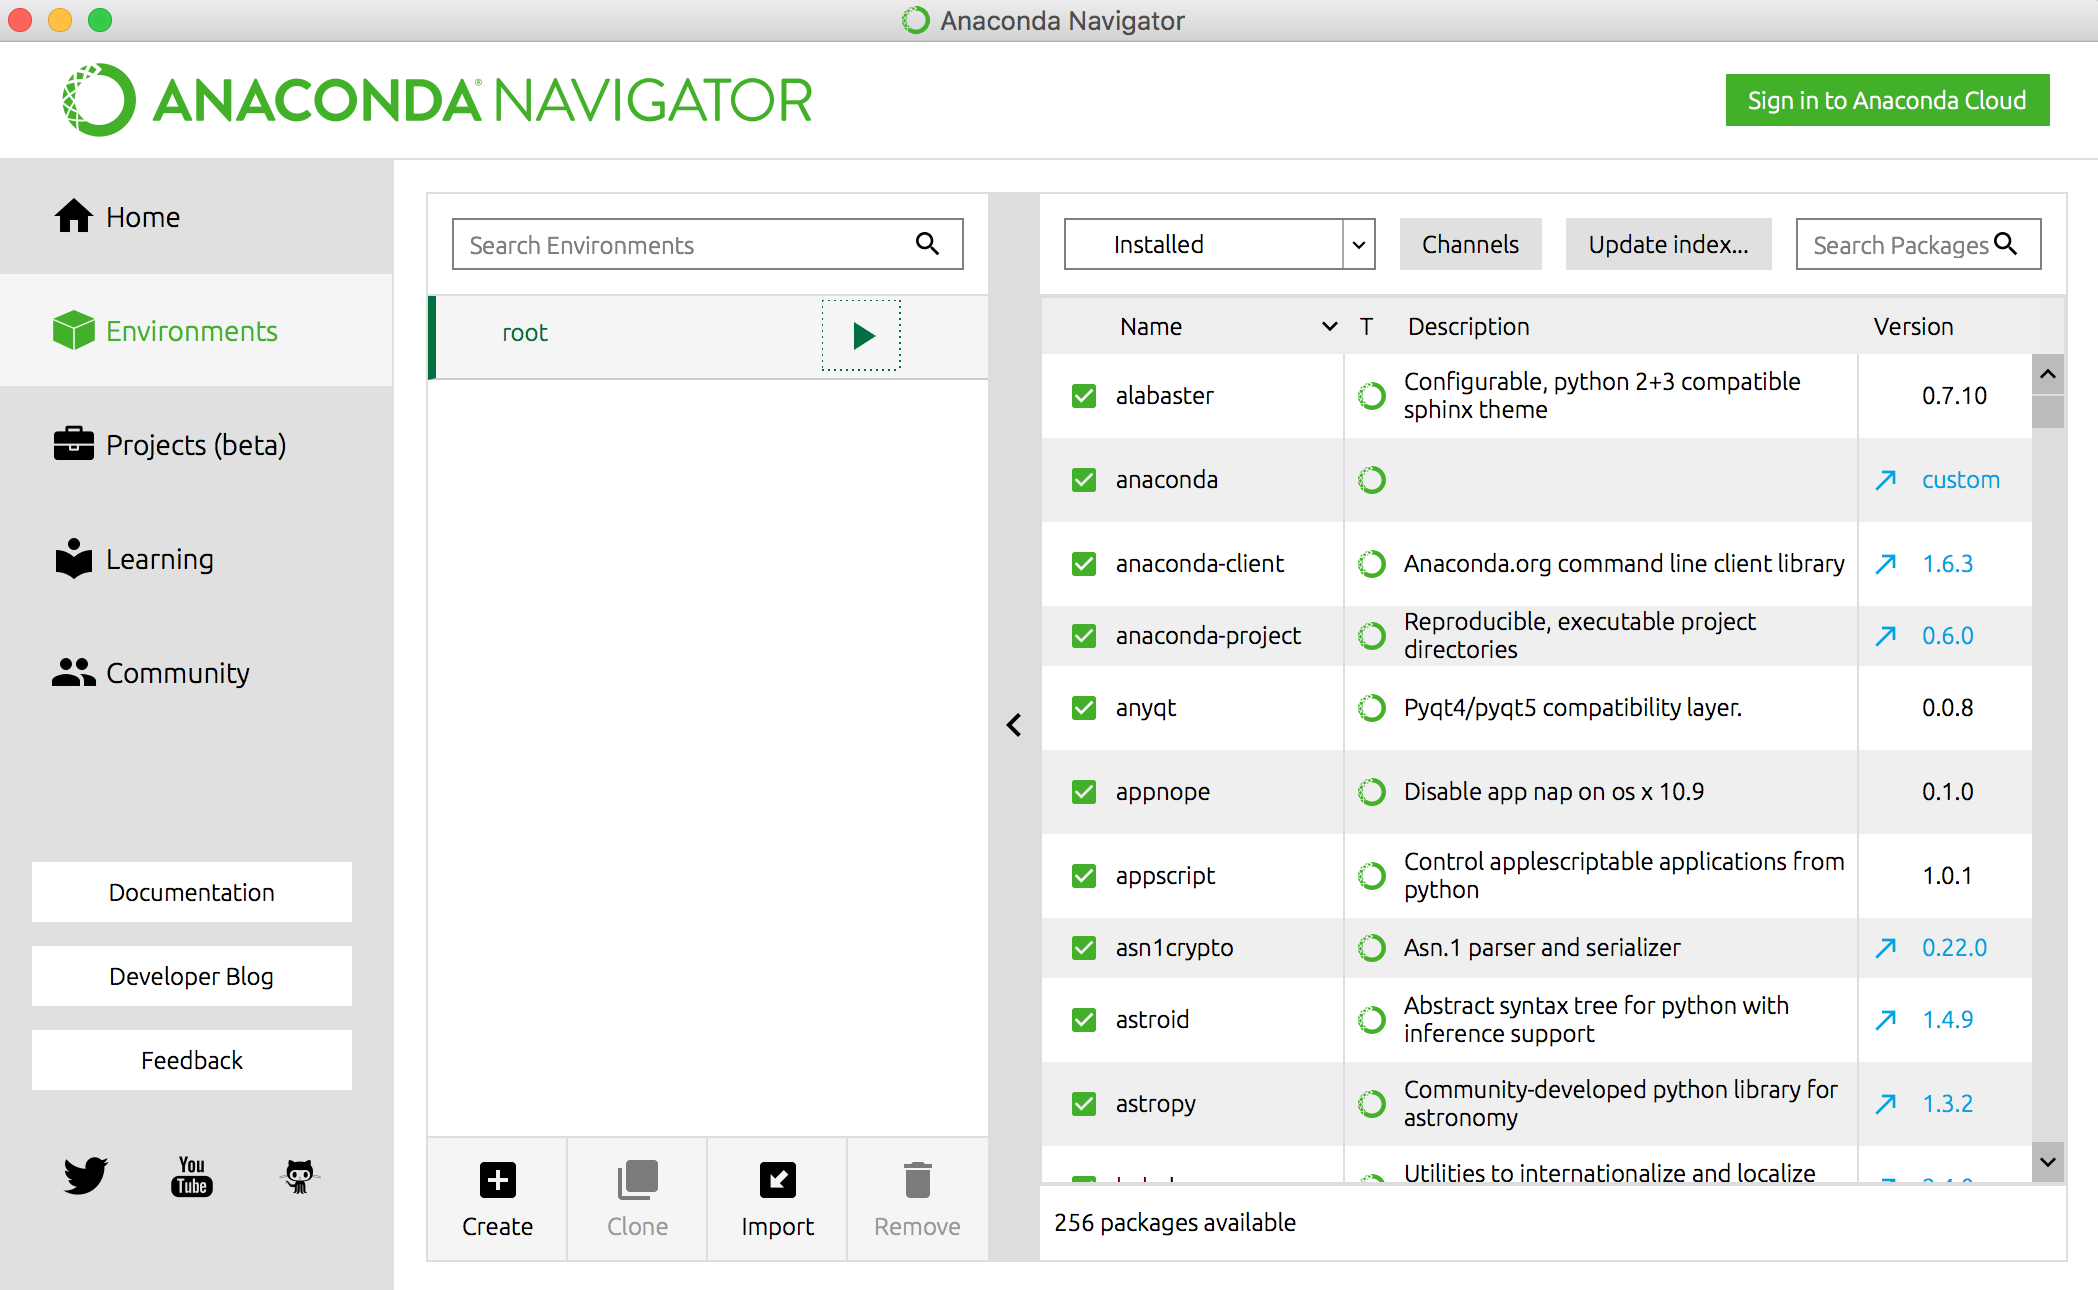
\includegraphics[width=12cm]{anaconda-env-win}
            \caption{The Environments window of the Anaconda-Navigator.}
            \label{anaconda-env-win}
        \end{figure}
        %
        \item Click the \textbf{Create} button on the bottom of the center panel. A new window titled ``Create new environment" will appear. (Figure \ref{anaconda-create-new-env-win})
        %
        \begin{figure}[h]
            \begin{center}
            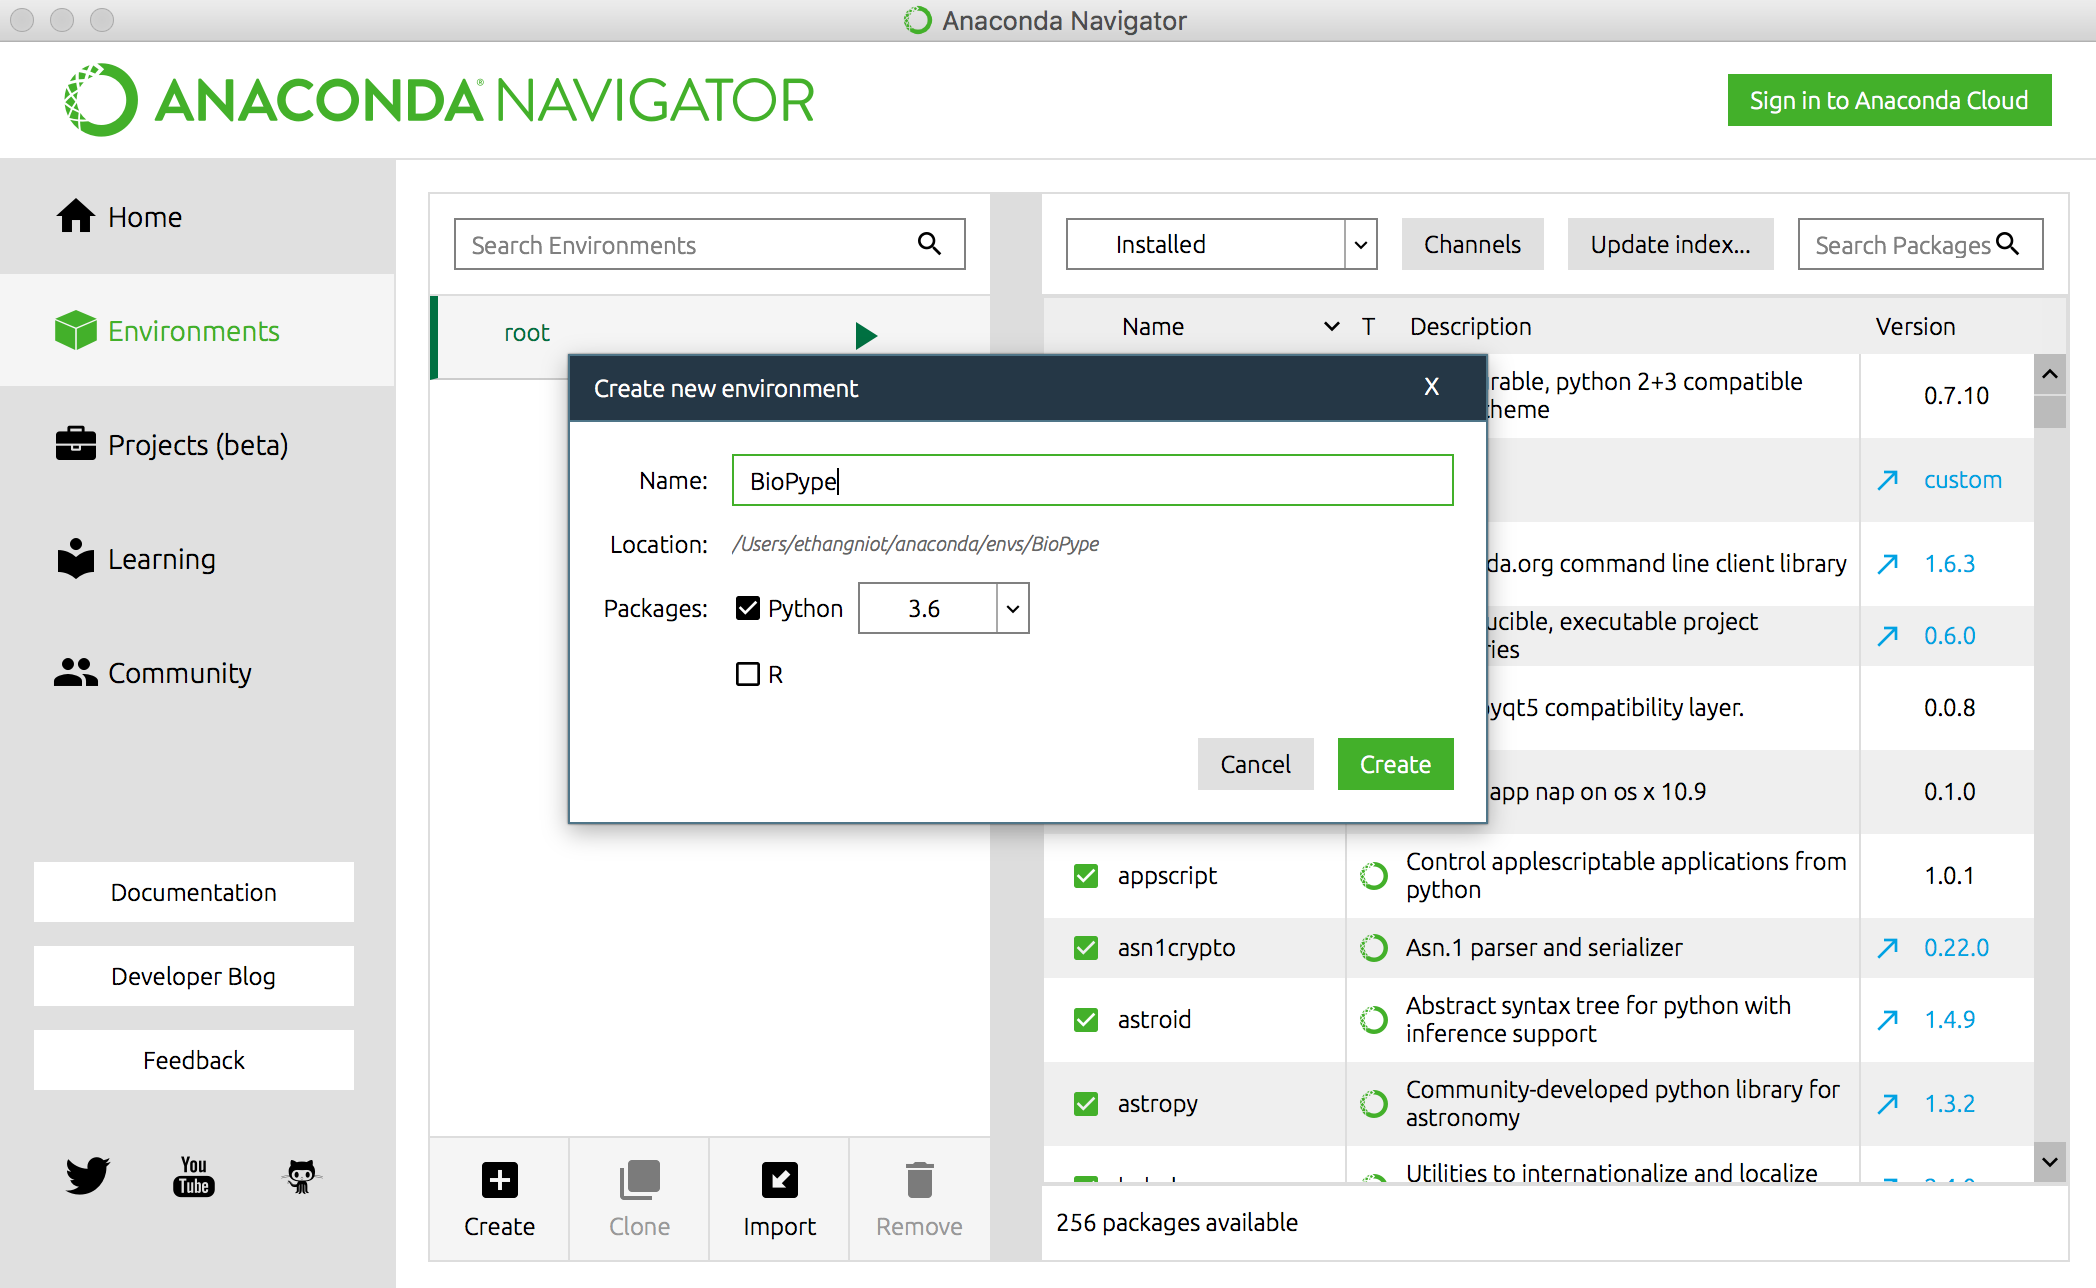
\includegraphics[width=12cm]{anaconda-create_new_env_win}
            \caption{The ``Create new environment" window.}
            \label{anaconda-create-new-env-win}
            \end{center}
        \end{figure}
        %
        \item Enter a \textbf{Name} for the environment. You may choose any name you want, but for the sake of this tutorial we will name the new environment ``BioPype".
        \item Select the box labeled \textbf{Python} next to the \textbf{Packages} heading.
        \item Choose the latest version of Python from the adjacent drop-down menu (Python 3.6 is the most current version at the time of this writing, so we choose \textbf{3.6}).
        \item Click the \textbf{Create} button within the ``Create new environment window".
    \end{enumerate}

\subsection{Install packages}
    \todo[inline]{Write blurb about what packages are.}
    \todo[inline]{Link to resource for further reading about packages.}
    \begin{enumerate}
        \item Change Anaconda's current environment from the \textbf{root} environment by selecting the \textbf{BioPype} tab in the middle panel of the Environments window.
        \item Click on the drop-down menu in the right-hand panel that says ``Installed" and change it to ``All".
        \item In the ``Search Packages" box, enter ``biopython". The search should return a package named ``biopython". Select the checkbox to the left of the name. (Figure \ref{anaconda-search-pack})
        \begin{itemize}
            \item A pair of green and red boxes (reading ``Apply" and ``Clear", respectively) will appear in the bottom-right of the window once the package is selected. Do not click these just yet. 
    %
    \begin{figure}[hbtp]
        \begin{center}
        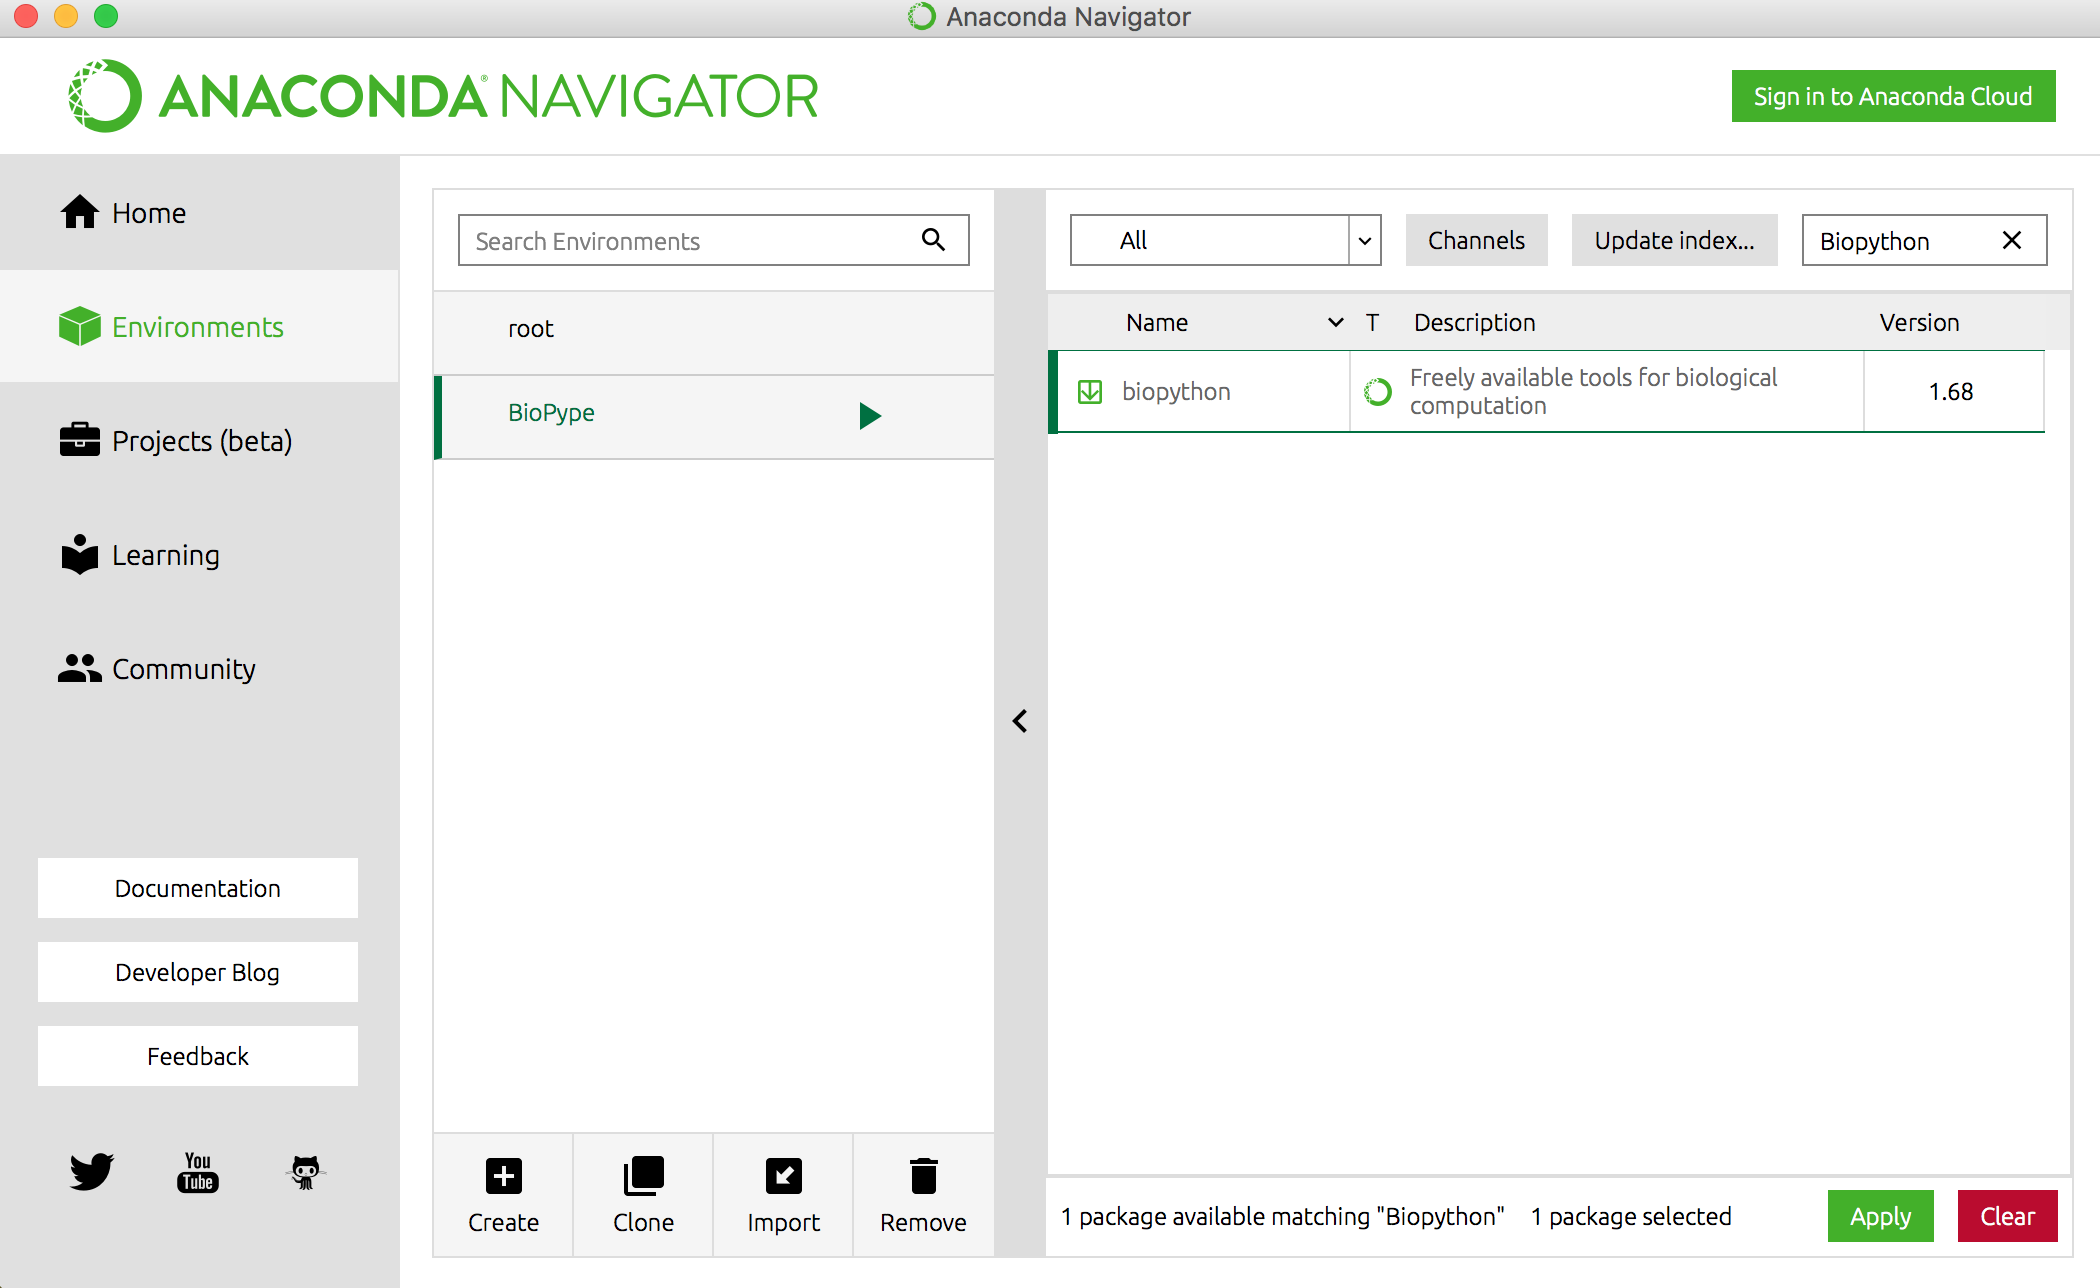
\includegraphics[width=12cm]{anaconda-search-pack}
        \caption{Searching for a package. When a package is selected, the checkbox next to the package's name will be green.}
        \label{anaconda-search-pack}
        \end{center}
    \end{figure}
    %
    \todo{Solve the issue with failing to center figures when they're on their own page}
        \end{itemize}
        \item Use the search bar to find and select the other packages listed in \autoref{tab:software}. Once all packages have been selected, click the green ``Apply" button in the bottom right corner of the window, then select ``Apply" again within the ``Install Packages" window that appears. (Figure \ref{anaconda-install-pack}) Anaconda will now install the selected packages.
    %
    \begin{figure}[hbtp]
        \begin{center}
        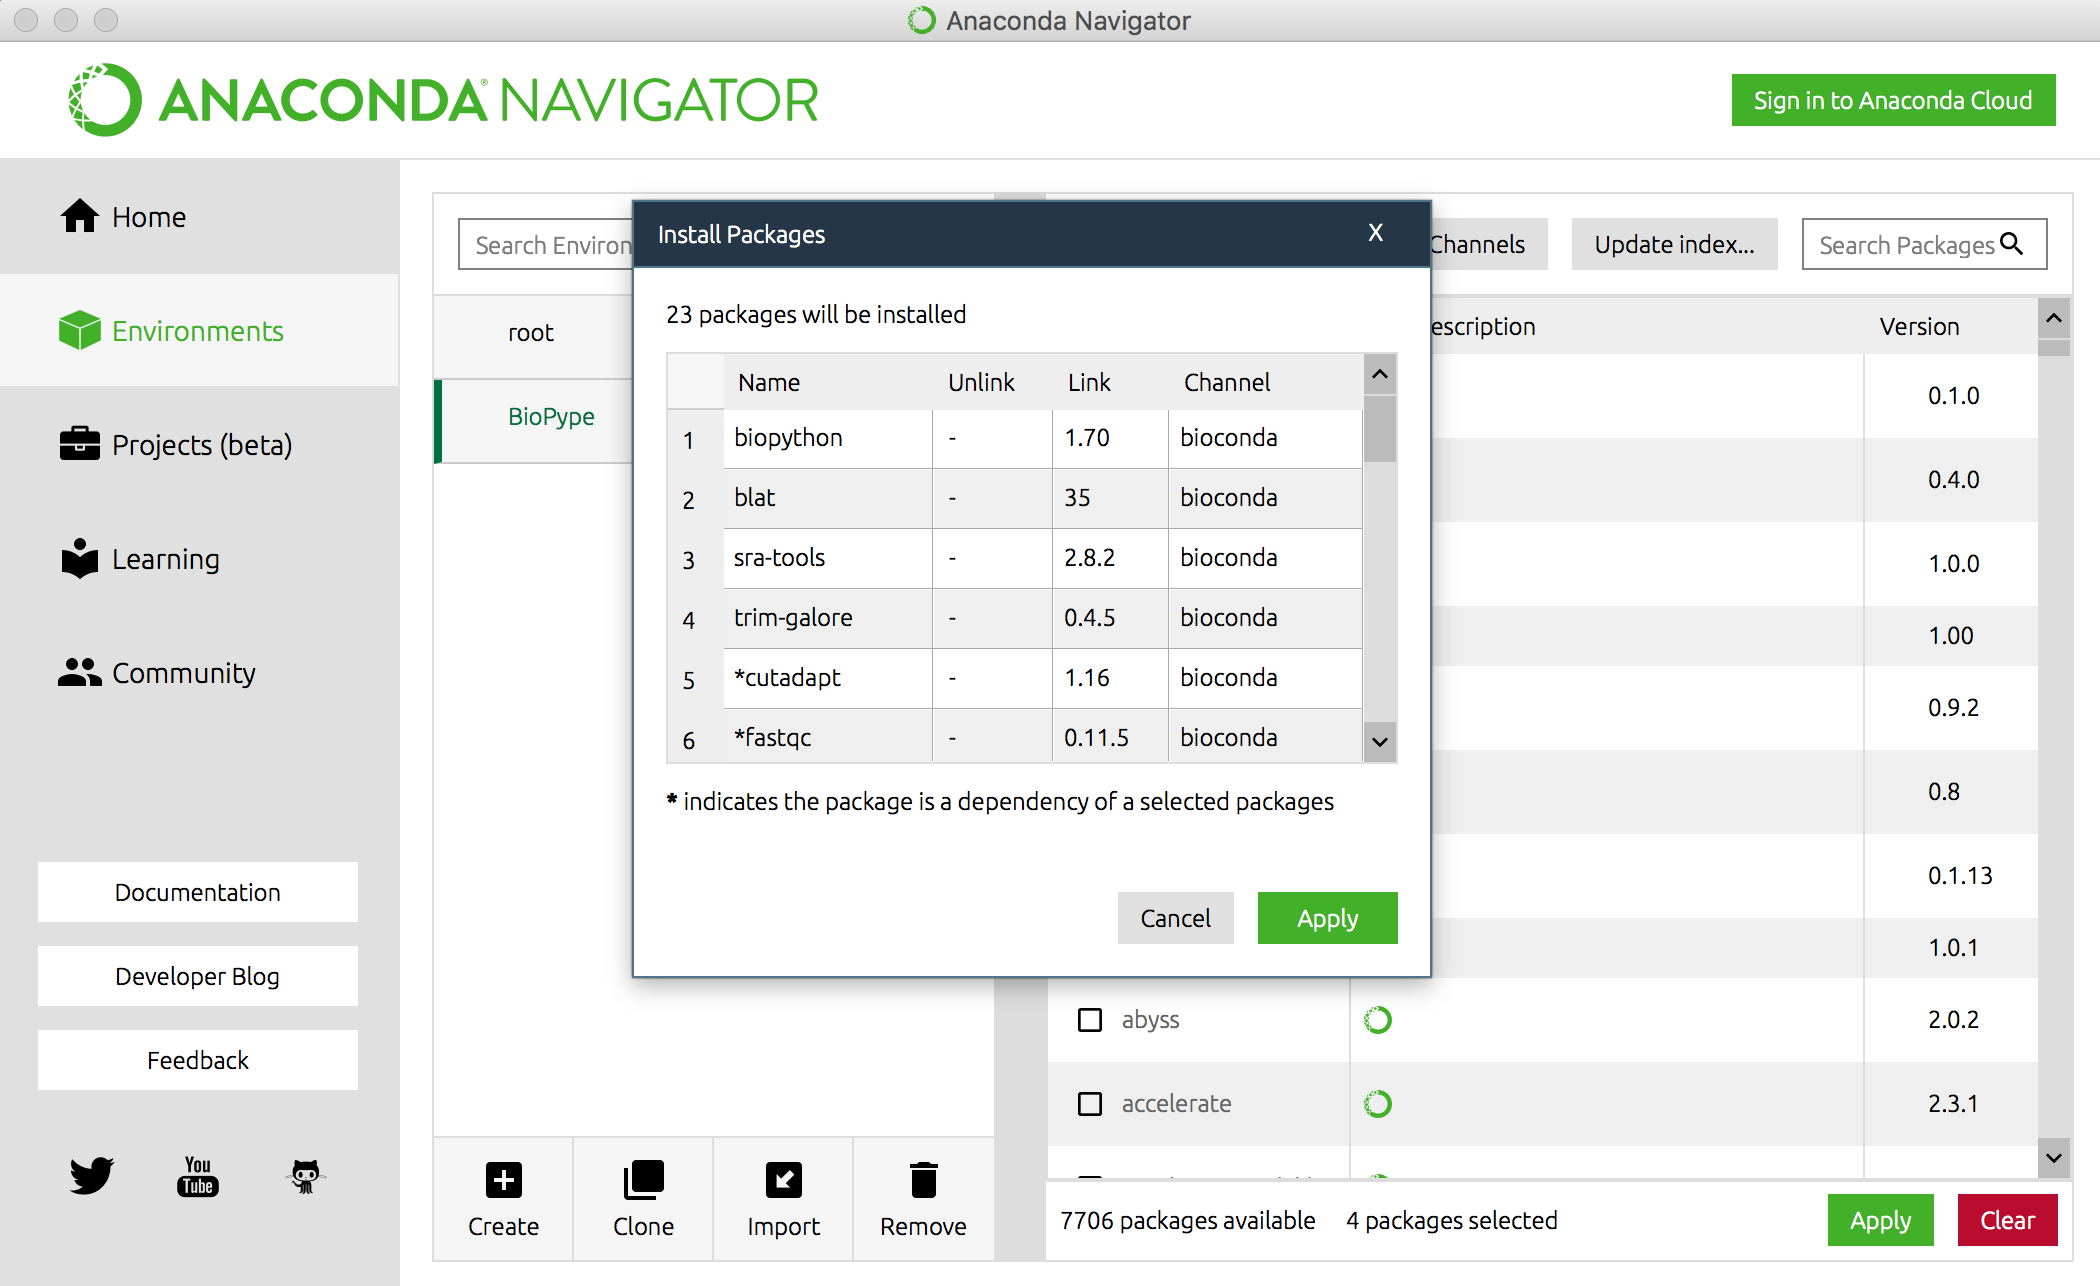
\includegraphics[width=12cm]{anaconda-install-pack}
        \caption{The window displaying the packages and dependencies that will be installed.}
        \label{anaconda-install-pack}
        \end{center}
    \end{figure}
    %
        \item \todo[inline]{Talk about setting up the sra-tools workspace (\url{https://trace.ncbi.nlm.nih.gov/Traces/sra/sra.cgi?view=toolkit_doc&f=std})}
        \item \todo[inline]{PYPIPER IS ONLY COMPATIBLE WITH MAC AND LINUX. Start by coding with just subprocess module commands. If the scripts work on Windows computers, then forget about using pypiper. But if the subprocess scripts don't work on windows, then we'll be developing exclusively for Mac anyways, so you could use pypiper without any worries. In that case, talk about installing pypiper here. OTHERWISE, delete this section.}
        \begin{enumerate}
            \item Open a terminal window in the BioPype environment by clicking the ``play" button on the BioPype environment tab and then selecting ``Open Terminal".
            \item Wait for the terminal window to finish opening. You'll know it's finished when you see \todo[inline]{show image of what the prompt looks like when it's done initializing.}
            \item Install \textbf{pypiper} by typing the following at the command prompt, followed by pressing return/enter:
            %
            \begin{lstlisting} [language=Python]
                pip install --user pypiper
            \end{lstlisting}
            %
            \item Check that the package was installed correctly by executing the following in the command prompt:
            %
            \begin{lstlisting} [language=Python]
                conda list
            \end{lstlisting}
            %
            This will generate a list of all the packages installed in the current environment. If you see the \textbf{pypiper} package listed, the installation was successful and you may skip the rest of this section. If not, proceed with the following steps.
            \item Execute the install command from step (c) again. This time, the Terminal should return a message similar to the one displayed in \todo[inline]{Reference the figure pypiper-already-installed}. The line that reads ``Requirement already satisfied: pypiper in ...." tells us the location where the package was (incorrectly) installed. 
            \missingfigure{pypiper-already-installed}
            \item Open a Terminal window, and navigate to the location indicated by the message from the previous step. For my example, I need to start at my home directory and walk through the following folders: .local | lib | python3.6 | site-packages. 
            \begin{itemize}
                \item The folders along the path to the pypiper installation may be hidden. On a Mac, these hidden folders are preceded by a ``." If the path to the pypiper installation includes hidden locations, reveal them by pressing ``Cmd + Shift + ." in the Finder window.
            \item Once you find the site-packages folder containing two pypiper folders \todo[inline]{reference figure pypiper-wrong-location}, copy those folders and their contents and paste them into the ~/anaconda/envs/BioPype/lib/python3.6/site-packages directory. The package should now be installed correctly. \missingfigure{pypiper-wrong-location} 
            \marginlabel{}
            \end{itemize}
        \end{enumerate}    
    \end{enumerate}

\subsection{Integrated Development Environment (IDE)}
\todo[inline]{Talk about choosing between PyCharm and other options}
%
\subsection{PATH}
\todo[inline]{(Talk about putting all the tools in the same path/directory)}
\section{Analysis Pipeline}
(Use figures to illustrate the stages of the pipeline)

\chapter{The Dataset}

In the previous chapter, we set up our machine so that it has all of the software BioPype needs in order to function.

In this chapter, we will use BioPype to download experimental data, and then prepare them for analysis via a process called 
``quality control".

    %
    \section{The Data}
        What experiment are the data from? 
        What was the study investigating? 
        Where did we find the data?



(Find dataset)

(Create script to automate download of data)

(Quality control protocols and how to make script for automated QC)

    %
    \section{Find Dataset}
        %
        \begin{enumerate}
            \item NCBI
            \item SRA database
            \item Look for WGS data
        \end{enumerate}
        %
    %
    \section{Download Dataset}
        %
        \begin{enumerate}
            \item Download RunInfo Table
            \item Create RunTable object from RunInfo Table file
            \item Use filtering methods of RunTable object to select data
        \end{enumerate}
    
        %
        \subsection{BioPype Workflow}
        
        %
        \subsection{Creating the code}
        
        %
    
    
    \section{Perform Quality Control on Dataset}



\chapter{Section 3: Relative Abundance Analysis}
(How to compare relative abundance of bacterial taxa between experimental conditions using QWRAP.)

\chapter{Section 4: Predict ORFs}
(how to predict the ORFs of the sequencing reads)

\chapter{Section 5: Create Non-redundant Gene Sets}
(How to create non-redundant gene sets using the predicted ORFs and what kind of information they provide)
(Align reads using BLAT)

\chapter{Section 6: Align Genes}

\chapter{Section 7: Get GenBank Accession Numbers}

\chapter{Section 8: Find COG Functional Classes}

\chapter{New Analysis}
(Walk user through analysis of new, untested dataset looking for age-related differences in patients with Inflammatory Bowel Disease.)

\chapter{TODO}
\begin{itemize}
    \item Talk about the IBD dataset in Chapter 3: Sample Information
    \item Fix the bibliography citations. Some work, some don't, and I'm not sure why.
    \item Put URLs in footnotes instead of appendix entries?
\end{itemize}

%
\begin{appendix}
\chapter{Web Links}
    \section{this is a test section}
    \label{test-label}
    \section{\url{http://nbviewer.jupyter.org/github/biocore/qiime/blob/1.9.1/examples/ipynb/illumina_overview_tutorial.ipynb}}
    \label{appendix:IlluminaOverTut}
    \section{\url{https://docs.qiime2.org/2018.2/tutorials/moving-pictures/}}
    \label{appendix:MovingPicTut}
    \section*{Link 3}

\chapter{Referenced Studies}
%https://www.ncbi.nlm.nih.gov/pubmed/21624126
\end{appendix}
%
\bibliographystyle{plain}
%
\bibliography{/Users/ethangniot/Documents/Bibtex/LU-microbiome_manual}

%%%%%%%%%%%
% When you define a \label outside a figure, a table, or other floating objects, the label points to the current section. In some cases, this behavior is not what you'd like and you'd prefer the generated link to point to the line where the \label is defined. This can be achieved with the command \phantomsection as in this example:

%The link location will be placed on the line below.
%\phantomsection
%\label{the_label}
%%%%%%%%%%



\end{document}
